% SGA 6, Exposición I: apertura y sección 1 en español, alineadas con la fuente.
% Alcance exacto: sga6_fr_r1/src/fr.tex, líneas 1624--1948.
% Las lecturas diplomáticas corregidas de forma transparente se conservan mediante \sisi.

\section*{Exposición I. Generalidades sobre las condiciones de finitud en las categorías derivadas}
\begin{center}
por L. Illusie
\end{center}

\subsection*{0. Introducción}
El objeto de las Exposiciones I a IV es desarrollar, con la generalidad conveniente en este Seminario, el formalismo de las condiciones de finitud en las categorías derivadas de los topos anillados.

Como se dijo en la Exp.\ 0, fue la necesidad de definir sobre esquemas arbitrarios « grupos de Grothendieck » con buenas propiedades de varianza lo que obligó a generalizar y flexibilizar las nociones de finitud utilizadas hasta ahora.

Una noción clásica como la de haz coherente sobre un espacio anillado \((X,\mathcal O_X)\) deja de tener interés en cuanto \(\mathcal O_X\) deja de ser coherente. Podría pensarse en sustituirla por la noción de presentación finita, pero esta presenta el inconveniente de que, en general, el núcleo de un epimorfismo de módulos de presentación finita ya no es de presentación finita. Se llega a una noción satisfactoria observando que, si \(\mathcal O_X\) es coherente, un haz coherente \(F\) no solo es de presentación finita, sino de \(n\)-presentación finita para todo \(n\in\mathbb N\); « \(n\)-presentación finita » significa que existe localmente una sucesión exacta
\[
  L_n\longrightarrow L_{n-1}\longrightarrow \ldots \longrightarrow L_0\longrightarrow F\longrightarrow 0,
\]
donde los \(L_i\) son libres de tipo finito. Sin suponer ya que el haz \(\mathcal O_X\) sea coherente, diremos que un \(\mathcal O_X\)-módulo \(F\) es \emph{pseudocoherente} si verifica la condición anterior, es decir, si es de \(n\)-presentación finita para todo \(n\). Entonces la noción de pseudocoherencia posee, respecto de las sucesiones exactas cortas, la misma propiedad de estabilidad que la noción de coherencia: si dos de los términos de una sucesión exacta corta de \(\mathcal O_X\)-módulos son pseudocoherentes, el tercero también lo es.

La noción anterior se generaliza fácilmente a los complejos de haces. Se dice que un \emph{complejo} \(F\) de \(\mathcal O_X\)-módulos es \emph{pseudocoherente} si es \(n\)-pseudocoherente para todo \(n\in\mathbb Z\); « \(n\)-pseudocoherente » significa que existe localmente un cuasi-isomorfismo \(L\to F\), donde \(L\) es un complejo acotado superiormente y con componentes libres de tipo finito en grado \(\geq n\). Para un complejo \(F\) concentrado en grado \(0\), es equivalente decir que \(F\) es pseudocoherente como complejo o como módulo.

La noción de complejo pseudocoherente posee excelentes propiedades de estabilidad, descritas en la Exp.\ I \S\S~1 y 2. En primer lugar, es una noción estable por isomorfismo en la categoría derivada \(\Db(X)\) de la categoría de los \(\mathcal O_X\)-módulos; más aún, si dos de los objetos de un triángulo distinguido de \(\Db(X)\) son pseudocoherentes, el tercero también lo es: en otros términos, la subcategoría plena \(\Db(X)_{\mathrm{coh}}\) de \(\Db(X)\) formada por los complejos pseudocoherentes es una subcategoría triangulada. Además, la pseudocoherencia se conserva por imagen inversa derivada y producto tensorial derivado. Cuando \(\mathcal O_X\) es coherente, decir que un complejo \(F\) es pseudocoherente significa simplemente que \(F\) tiene cohomología localmente acotada superiormente y que todos sus \(\underline H^i(F)\) son coherentes.

Si \(\mathcal O_X\) es un haz de anillos locales regulares, todo \(\mathcal O_X\)-módulo coherente \(F\) admite localmente una resolución izquierda \emph{finita} por módulos libres de tipo finito, es decir, existe localmente una sucesión exacta
\[
  0\longrightarrow L_n\longrightarrow \ldots \longrightarrow L_0\longrightarrow F\longrightarrow 0,
\]
donde los \(L_i\) son libres de tipo finito. Por tanto, cuando \(\mathcal O_X\) es un haz cualquiera de anillos locales, es natural interesarse por los módulos que gozan de la propiedad anterior. Tales módulos se llaman \emph{perfectos}. Más generalmente, se dice que un \emph{complejo} \(F\) de \(\mathcal O_X\)-módulos es \emph{perfecto} si existe localmente un cuasi-isomorfismo \(L\to F\), donde \(L\) es un complejo acotado y con componentes libres de tipo finito. En la Exp.\ I \S~3 se demuestra que la subcategoría plena \(\Db(X)_{\mathrm{parf}}\) de \(\Db(X)\), formada por los complejos perfectos, es, al igual que \(\Db(X)_{\mathrm{coh}}\), una subcategoría triangulada, « estable » por imagen inversa derivada y producto tensorial derivado. Evidentemente, se tiene
\[
  \Db(X)_{\mathrm{parf}}\subset\Db(X)_{\mathrm{coh}},
\]
pero la inclusión es estricta en general. La pseudocoherencia puede redefinirse « por paso al límite » a partir de la perfectitud: un complejo \(F\) es pseudocoherente si y solo si, para todo \(n\in\mathbb Z\), \(F\) puede ser « aproximado localmente hasta el orden \(n\) por un complejo perfecto », con lo cual se quiere decir que existe localmente un triángulo distinguido
\[
\begin{tikzcd}
& R \arrow[dl] &\\
L \arrow[rr] && F \arrow[ul]
\end{tikzcd}
\]
donde \(L\) es perfecto y \(R\) es acíclico en grado \(\geq n\). Recíprocamente, la perfectitud se recupera a partir de la pseudocoherencia gracias a una condición adicional de regularidad: un complejo es perfecto si y solo si es pseudocoherente y localmente de tor-dimensión finita (Exp.\ I \S~5). Se recupera así el hecho de que, si los anillos locales son regulares, todo haz coherente es perfecto; más generalmente, todo complejo pseudocoherente de cohomología localmente acotada es perfecto.

La pseudocoherencia y la perfectitud son las dos nociones fundamentales de finitud con las que trabajaremos en este Seminario. Los §§~1 a 5 de la Exposición I están dedicados a su definición y al establecimiento de sus propiedades elementales de estabilidad. Para ello solo se utilizan dos o tres propiedades locales de la categoría de los módulos libres de tipo finito respecto de la categoría de todos los módulos. Por ello resulta conveniente~-- y útil, en particular en la Exp.\ II~- axiomatizar la situación, introduciendo una noción de pseudocoherencia (respectivamente, de perfectitud) en una categoría fibrada sobre un sitio, relativamente a una subcategoría fibrada que verifica condiciones convenientes.

Los §§~6 a 8 de la Exp.\ I generalizan a los complejos perfectos cierto número de nociones bien conocidas para los haces localmente libres de tipo finito: rango, dualidad y traza de un endomorfismo.

En la Exp.\ II se examina el problema de la «~existencia de resoluciones globales~»: ¿bajo qué condiciones, sobre un topos anillado \((X,\mathcal O_X)\), un complejo pseudocoherente (respectivamente, perfecto) es \emph{globalmente} isomorfo en \(\Db(X)\) a un complejo de módulos localmente libres de tipo finito? La importancia de esta cuestión reside esencialmente en que, por el momento, no se sabe generalizar a los complejos perfectos ciertas construcciones usuales sobre los módulos localmente libres, como las potencias exteriores y simétricas y las clases de Chern (para más detalles sobre este asunto, véase la Exp.\ XIV). Por ello conviene disponer de criterios suficientes y manejables para la existencia de resoluciones globales, lo que permite reducir ciertas cuestiones sobre los complejos pseudocoherentes (respectivamente, perfectos) a cuestiones análogas sobre los haces localmente libres de tipo finito. Tales criterios se dan en la Exp.\ II.

Se demuestra, en particular, que existen resoluciones globales en los casos siguientes: \(X\) es el topos de Zariski de un esquema afín, o, más generalmente, de un esquema cuasicompacto que posee un haz invertible amplio, o incluso una familia amplia de haces invertibles en el sentido de Kleiman (por ejemplo, un esquema regular); o bien \(X\) es el topos de los haces de conjuntos sobre un espacio topológico compacto y \(\mathcal O_X\) el haz de las funciones continuas con valores complejos. A modo de ilustración~-- y para poner de manifiesto la flexibilidad de las nociones introducidas~-- se da en un apéndice una definición «~puramente de haces~» del índice de una familia de operadores elípticos.

La Exp.\ III estudia la estabilidad de las condiciones de finitud por imagen directa derivada. Para obtener enunciados razonables, es preciso «~relativizar~» las nociones de pseudocoherencia y perfectitud. Aquí nos situamos en el marco de los esquemas ordinarios, lo que basta para el Seminario, pero no cabe duda de que, tarde o temprano, habrá que desarrollar una teoría análoga para los esquemas o espacios analíticos relativos. Sea \(p:X\to S\) un \(S\)-esquema localmente de tipo finito y sea \(F\) un complejo de \(\mathcal O_X\)-módulos; se dice que \(F\) es \emph{pseudocoherente} (\emph{respectivamente, perfecto}) \emph{relativamente a} \(p\) si localmente se puede sumergir \(X\) (mediante una inmersión cerrada) en un \(S\)-esquema liso \(X'\), de manera que \(F\), prolongado por cero sobre \(X'\), sea pseudocoherente (respectivamente, perfecto). La noción de pseudocoherencia relativamente a \(p\) es especialmente interesante cuando \(S\) no es localmente noetheriano, pues en caso contrario coincide con la noción ordinaria de pseudocoherencia. Por otra parte, como cabe esperar, decir que \(F\) es perfecto rel.\ a \(p\) equivale a decir que \(F\) es pseudocoherente rel.\ a \(p\) y localmente de tor-dimensión finita rel.\ a \(p\) (es decir, rel.\ al haz de anillos \(p^{-1}(\mathcal O_S)\)).

El teorema central de la Exp.\ III es el \emph{teorema de finitud}, que afirma (en una forma algo más precisa) que, si \(f:X\to Y\) es un morfismo \emph{propio} de \(S\)-esquemas localmente de tipo finito, el funtor \(Rf_*\) transforma complejos pseudocoherentes rel.\ a \(S\) en complejos pseudocoherentes rel.\ a \(S\); este teorema es en realidad una conjetura, pero se demuestra, no obstante, en los dos casos particulares siguientes: a)~\(S\) es localmente noetheriano; b)~\(f\) es proyectivo; por desgracia, parece que la extensión al caso general es del mismo orden de dificultad que el teorema análogo en Geometría Analítica («~teorema~» de Grauert). Combinando el teorema de finitud con una fórmula esencialmente trivial llamada \emph{fórmula de proyección}, se obtienen criterios manejables para la estabilidad de la perfectitud relativa por imagen directa. Se recuperan, como corolario, los «~teoremas de continuidad y semicontinuidad de Grauert~» (EGA III 7.6).

La Exp.\ IV traduce al lenguaje de los «~grupos de Grothendieck~» los resultados de las Exp.\ I a III. Sobre un topos anillado \((X,\mathcal O_X)\), se denota por \(K^\bullet(X)\) (respectivamente, \(K_\bullet(X)\)) el «~grupo de Grothendieck~» de la categoría de los complejos perfectos y de tor-dimensión finita (respectivamente, pseudocoherentes y de cohomología acotada). El grupo \(K^\bullet(X)\) es un anillo, y \(K_\bullet(X)\) un módulo sobre \(K^\bullet(X)\). \(K^\bullet\) es un funtor contravariante (como sugiere el punto superior), mientras que \(K_\bullet\) es un funtor covariante para los morfismos propios y pseudocoherentes (de esquemas o de espacios analíticos, y a reserva de que se disponga del teorema de finitud\dots). Existen también varianzas inusuales: covarianza de \(K^\bullet\) y contravarianza de \(K_\bullet\), para morfismos que satisfacen hipótesis convenientes de regularidad. Por último, los criterios de globalización de la Exp.\ II permiten establecer el vínculo con los «~grupos de Grothendieck~» definidos ingenuamente a partir de los haces coherentes o de los haces localmente libres de tipo finito.

\section*{1. Definiciones preliminares}

\subsection*{1.1. Categorías fibradas con fibras aditivas (respectivamente, abelianas, respectivamente, trianguladas)}

\textbf{1.1.1.} Sea \(S\) una categoría, y sea \(\mathcal C\) una \(S\)-categoría fibrada (SGA 1 VI 6.1) cuyas fibras son categorías aditivas (respectivamente, trianguladas). Diremos que \(\mathcal C\) es una \emph{\(S\)-categoría aditiva} (\emph{respectivamente, triangulada}) (o que \(\mathcal C\) es aditiva (respectivamente, triangulada) sobre \(S\)) si, para toda flecha \(f:X\to Y\) de \(S\), el funtor de imagen inversa (determinado salvo isomorfismo único) \(f^*:\mathcal C_Y\longrightarrow \mathcal C_X\) es aditivo (respectivamente, exacto). Diremos que \(\mathcal C\) es una \(S\)-categoría \emph{abeliana} si \(\mathcal C\) es una \(S\)-categoría aditiva con fibras abelianas, y que \(\mathcal C\) es una \(S\)-categoría abeliana \emph{plana} si, además, los funtores de imagen inversa son exactos.

\textbf{1.1.2.} Sea \(\mathcal C\) una \(S\)-categoría triangulada. Se define, por ejemplo mediante un clivaje de \(\mathcal C\) (SGA 1 VI 7.1), una \(S\)-categoría fibrada \(\Trc(\mathcal C)\) cuya fibra en cada \(X\in \ob(S)\) es la categoría \(\Trc(\mathcal C_X)\) de los triángulos distinguidos de \(\mathcal C_X\).

\textbf{1.1.3.} Sean \(\mathcal C\) y \(\mathcal C'\) dos \(S\)-categorías aditivas (respectivamente, trianguladas), y \(F:\mathcal C\to\mathcal C'\) un funtor. Se dice que \(F\) es un \emph{\(S\)-funtor aditivo} (\emph{respectivamente, exacto}) si \(F\) es un \(S\)-funtor cartesiano aditivo (respectivamente, exacto) sobre cada fibra.



% Definiciones adicionales de macros
\providecommand{\cC}{\mathcal C}
\providecommand{\cD}{\mathcal D}
\providecommand{\cK}{\mathcal K}
\providecommand{\cO}{\mathcal O}
\providecommand{\cS}{\mathcal S}
\providecommand{\Cpx}{\mathrm C}
\providecommand{\Kpx}{\mathrm K}
\providecommand{\Dpx}{\mathrm D}
\providecommand{\D}{\mathrm D}
\providecommand{\Ho}{\mathrm H}
\providecommand{\RHom}{\mathrm R\!\operatorname{Hom}}
\providecommand{\Ob}{\operatorname{ob}}
\providecommand{\Coker}{\operatorname{Coker}}
\providecommand{\Ker}{\operatorname{Ker}}
\providecommand{\Im}{\operatorname{Im}}
\providecommand{\Hom}{\operatorname{Hom}}
\providecommand{\Cone}{\operatorname{Cone}}
\providecommand{\id}{\operatorname{Id}}
\providecommand{\qis}{\xrightarrow{\sim}}


Si \(\mathcal C\) y \(\mathcal C'\) son \(S\)-categorías trianguladas y \(F\) es un \(S\)-funtor exacto, entonces \(F\) define un \(S\)-funtor cartesiano \(\Trc(\mathcal C)\longrightarrow \Trc(\mathcal C')\).

\textbf{1.1.4.} Sea \(\mathcal C\) una \(S\)-categoría triangulada, y sea \(\mathcal C'\) una sub-\(S\)-categoría fibrada plena de \(\mathcal C\). Se dice que \(\mathcal C'\) es una \emph{sub-\(S\)-categoría triangulada} de \(\mathcal C\) si, para todo \(X\in\Ob S\), \(\mathcal C'_X\) es una subcategoría triangulada de \(\mathcal C_X\) ([V] cap.\ I \S~1 2.3).

\textbf{1.1.5.} Sea \(\mathcal C\) una \(S\)-categoría aditiva. Se define (SGA 4 XVII 2.2, 2.4) una \(S\)-categoría aditiva (respectivamente, triangulada) \(\Cpx(\mathcal C)\) (respectivamente, \(\Kpx(\mathcal C)\)), cuya fibra en \(X\in\Ob S\) es la categoría \(\Cpx(\mathcal C_X)\) (respectivamente, \(\Kpx(\mathcal C_X)\)) de los complejos\footnote{con diferencial de grado \(+1\).} (respectivamente, complejos «~módulo homotopía~») de \(\mathcal C_X\). Si \(\mathcal C\) es una \(S\)-categoría abeliana plana, se define (loc.\ cit.) una \(S\)-categoría triangulada \(\Dpx(\mathcal C)\), cuya fibra en \(X\in\Ob S\) es la categoría derivada \(\Dpx(\mathcal C_X)\); si \(f:X\to Y\) es una flecha de \(S\), denotaremos por \(f^*:\Dpx(\mathcal C_Y)\longrightarrow \Dpx(\mathcal C_X)\) el funtor de imagen inversa, que se deduce de \(f^*:\Kpx(\mathcal C_Y)\longrightarrow \Kpx(\mathcal C_X)\) por simple paso al cociente\footnote{\sisi{si \(a\in\Ob \Dpx(\mathcal C_Y)\) (respectivamente, \(F/\Dpx(\mathcal C_Y)\)), escribiremos a menudo, abreviadamente, \(a_X\) en lugar de \(f^*(a)\).}{si \(a\in\Ob \Kpx(\mathcal C_Y)\) (respectivamente, \(a\in\Ob \Dpx(\mathcal C_Y)\)), escribiremos a menudo, abreviadamente, \(a_X\) en lugar de \(f^*(a)\).}}. Se definen sub-\(S\)-categorías trianguladas plenas \(\Kpx^*(\mathcal C)\) (respectivamente, \(\Dpx^*(\mathcal C)\)) \((*=+,-,b)\) mediante las condiciones habituales de grado. % Canon SGA-SRC-001475

\textbf{1.2.} \emph{Terminología.} Sean \(S\) un sitio, \(\mathcal C\) una \(S\)-categoría abeliana plana (1.1), y \(\mathcal C_0\) una sub-\(S\)-categoría fibrada estrictamente plena.

Sea \(F\in\Ob\mathcal C_X\), para \(X\in\Ob S\). El conjunto de los \(f:U\to X\) de \(S_{/X}\) tales que existe un epimorfismo \(E\longrightarrow f^*F\), con \(E\in\Ob\mathcal C_{0,U}\), es un tamiz de \(X\). Si este es cubriente, diremos que \(F\) es de \(\mathcal C_0\)-\emph{tipo finito} (o simplemente de tipo finito, si no hay riesgo de confusión).

Diremos que \(\mathcal C_0\) es \emph{localmente estable por núcleos de epimorfismos} si se verifica la condición siguiente: para todo \(X\in\Ob S\) y todo epimorfismo \(u:E\longrightarrow F\) de \(\mathcal C_X\), con \(E\) y \(F\in\Ob\mathcal C_{0,X}\), el núcleo de \(u\) está localmente en \(\mathcal C_0\) (es decir, el conjunto de los \(f:U\to X\) de \(S_{/X}\) tales que \(f^*\Ker(u)\in\Ob\mathcal C_{0,U}\) es un refinamiento de \(X\)).

Mediante el procedimiento estándar de descomponer una sucesión exacta larga en sucesiones exactas cortas, se ve que la condición anterior equivale a la condición siguiente, en apariencia más fuerte: para todo \(X\in\Ob S\) y toda sucesión exacta de \(\mathcal C_X\)
\begin{equation}\tag{*}
  0\longrightarrow E^0\longrightarrow E^1\longrightarrow\ldots\longrightarrow E^n\longrightarrow 0
\end{equation}
con \(E^i\in\Ob\mathcal C_{0,X}\) para \(1\leq i\leq n\), \(E^0\) está localmente en \(\mathcal C_0\).

Diremos que \(\mathcal C_0\) es \emph{localmente cuasiestable por núcleos de epimorfismos} si, para toda sucesión exacta como \((*)\), \(E^0\) es de \(\mathcal C_0\)-tipo finito.

Por otra parte, diremos que \(\mathcal C_0\) es \emph{localmente levantable en} \(\mathcal C\) si, para todo \(X\in\Ob S\), todo epimorfismo \(u:E\longrightarrow F\) de \(\mathcal C_X\), con \(F\in\Ob\mathcal C_{0,X}\), admite localmente una sección. Para que \(\mathcal C_0\) sea localmente levantable en \(\mathcal C\), es necesario y suficiente que, para todo diagrama de \(\mathcal C_X\) (\(X\in\Ob S\))
\[
\begin{tikzcd}
& H \arrow[d]\\
E \arrow[r,"u"] & F
\end{tikzcd}
\]
donde \(u\) es un epimorfismo y \(H\in\Ob\mathcal C_0\), el conjunto de los \(U\) sobre \(X\) tales que existe un diagrama conmutativo
\[
\begin{tikzcd}
& H_U \arrow[d] \arrow[dl,"\sisi{u}{v}"']\\
E_U \arrow[r,"\sisi{U}{u_U}"] & F_U
\end{tikzcd}
\]
sea un refinamiento de \(X\).

Diremos que \(\mathcal C_0\) es \emph{localmente cuasilevantable en} \(\mathcal C\) si se verifica la condición más débil siguiente: para todo \(X\in\Ob S\), y todo epimorfismo \(u:E\longrightarrow F\) de \(\mathcal C_X\), con \(F\in\Ob\mathcal C_{0,X}\), el conjunto de los \(f:U\to X\) de \(S_{/X}\) tales que existe \(v:F'\longrightarrow f^*E\), con \(F'\in\Ob\mathcal C_{0,U}\), tal que \(f^*(u)v\) sea un epimorfismo, es un refinamiento de \(X\). Esta condición equivale a la siguiente: para todo diagrama de \(\mathcal C_X\)
\[
\begin{tikzcd}
& H \arrow[d]\\
E \arrow[r,"u"] & F ,
\end{tikzcd}
\]
donde \(u\) es un epimorfismo y \(H\in\Ob\mathcal C_0\), el conjunto de los \(U\) sobre \(X\) tales que existe un diagrama conmutativo
\[
\begin{tikzcd}
G \arrow[r,"v"] \arrow[d] & H_U \arrow[d]\\
E_U \arrow[r,"u_U"] & F_U
\end{tikzcd}
\]
con \(G\in\Ob\mathcal C_0\) y \(v\) un epimorfismo, es un refinamiento de \(X\).

Si \(S\) es un sitio caótico, por ejemplo el sitio puntual (un objeto, un morfismo), omitiremos el adverbio «~localmente~» en las definiciones anteriores.

\subsection*{1.3. Ejemplos}

\textbf{a)} Sean \(S\) un sitio puntual, \(A\) un anillo, y \(\mathcal C\) la categoría de los \(A\)-módulos izquierdos. La subcategoría plena \(\mathcal C_0\) de \(\mathcal C\), formada por los \(A\)-módulos (izquierdos) proyectivos de tipo finito, es estable por núcleos de epimorfismos y levantable en \(\mathcal C\); un \(A\)-módulo es de \(\mathcal C_0\)-tipo finito si y solo si es de tipo finito en el sentido ordinario. La subcategoría plena \(\mathcal C_1\) de \(\mathcal C\), formada por los \(A\)-módulos de tipo finito, es cuasilevantable en \(\mathcal C\) (pero no levantable en general); si \(A\) es noetheriano, \(\mathcal C_1\) es estable por núcleos de epimorfismos. La subcategoría plena \(\mathcal C'_0\) de \(\mathcal C\), formada por los \(A\)-módulos libres de tipo finito, es levantable en \(\mathcal C\) y cuasiestable (no estable en general) por núcleos de epimorfismos.

\textbf{b)} Sean \((S,\mathcal O_S)\) un espacio anillado por anillos locales, \(S\) el sitio de los abiertos de \(S\), y \(\mathcal C\) la \(S\)-categoría fibrada (e incluso escindida (SGA 1 VI 9)) definida por el funtor \(U\longmapsto\) (categoría de los \(\mathcal O_U\)-módulos izquierdos); \(\mathcal C\) es una \(S\)-categoría abeliana plana (1.1). Sea \(\mathcal C_0\) la sub-\(S\)-categoría aditiva estrictamente plena de \(\mathcal C\) definida por \(U\longmapsto\) (categoría de los \(\mathcal O_U\)-módulos libres de tipo finito). Un \(\mathcal O_S\)-módulo \(M\) es localmente de \(\mathcal C_0\)-tipo finito si y solo si \(M\) es de tipo finito en el sentido ordinario (EGA \(0_{\mathrm I}\) 5.2). De (EGA \(0_{\mathrm I}\) 5.2.7 y 5.4.9) resulta que \(\mathcal C_0\) es localmente estable por núcleos de epimorfismos y localmente levantable en \(\mathcal C\).

\textbf{c)} Sean \(G\) un grupo, \(S\) el topos de los \(G\)-conjuntos (SGA 4 V 3.11), \(k\) un cuerpo (considerado como anillo constante de \(S\)), y \(\mathcal C\) la \(S\)-categoría escindida definida por el funtor \(U\longmapsto\) (categoría de los \(k_U\)-módulos izquierdos); \(\mathcal C\) es una \(S\)-categoría abeliana plana. Sea \(\mathcal C_0\) la sub-\(S\)-categoría aditiva estrictamente plena de \(\mathcal C\), definida por \(U\longmapsto\) (categoría de los \(k_U\)-módulos libres de tipo finito).
Como la localización en \(S\) equivale a olvidar las operaciones de \(G\), está claro que un \(G\)-\(k\)-módulo \(M\) es localmente de \(\mathcal C_0\)-tipo finito si y solo si \(M\) tiene dimensión finita como espacio vectorial sobre \(k\), y que \(\mathcal C_0\) es localmente estable por núcleos de epimorfismos y localmente levantable en \(\mathcal C\).

Se deja al lector la tarea de considerar la variante «~galoisiana~» de c), donde \(G\) es un grupo profinito y \(S\) el topos de los conjuntos sobre los que \(G\) actúa continuamente.

De hecho, los ejemplos b) y c) son casos particulares del ejemplo siguiente:

d) Sean \((S,\mathcal O_S)\) un topos anillado (cf. SGA 4 IV 2.10)\footnote{\(\mathcal O_S\) es aquí un anillo de \(S\), con elemento unidad, pero no necesariamente conmutativo.}, y \(\mathcal C\) la \(S\)-categoría escindida definida por \(U\longmapsto\) (categoría de los \(\mathcal O_U\)-módulos izquierdos); \(\mathcal C\) es una \(S\)-categoría abeliana plana. Sea \(\mathcal C_0\) la sub-\(S\)-categoría aditiva estrictamente plena de \(\mathcal C\), definida por \(U\longmapsto\) (categoría de los \(\mathcal O_U\)-módulos libres de tipo finito). Un \(\mathcal O_S\)-módulo localmente de \(\mathcal C_0\)-tipo finito se dirá simplemente de \emph{tipo finito}. La categoría \(\mathcal C_0\) es localmente cuasiestable por núcleos de epimorfismos y localmente levantable en \(\mathcal C\), como resulta del

\textbf{Lema 1.3.1.} \emph{Sea \(P\) un \(\mathcal O_S\)-módulo. Las condiciones siguientes son equivalentes}:
\begin{enumerate}[label=(\roman*)]
\item \emph{\(P\) es de tipo finito y el funtor \(\Hom(P,.)\) es exacto};
\item \emph{\(P\) es de tipo finito y todo epimorfismo \(M\to P\) admite localmente una sección};
\item \emph{\(P\) es localmente factor directo de un módulo libre de tipo finito}.
\end{enumerate}
La demostración es inmediata y se deja como ejercicio al lector.

\subsection*{1.4. Un lema de «~prolongación~» (cf. EGA \(0_{\mathrm{III}}\) 11.9.1)}

\textbf{Proposición 1.4.1.} Sean \(\sisi{S}{\mathcal S}\) un sitio, \(\mathcal C\) una \(\sisi{S}{\mathcal S}\)-categoría abeliana plana (1.1), y \(\mathcal C_0\) una sub-\(\sisi{S}{\mathcal S}\)-categoría aditiva (1.1), estrictamente plena, de \(\mathcal C\); se supone que \(\mathcal C_0\) es localmente cuasilevantable en \(\mathcal C\) (1.2). Sea \(S\in\Ob \sisi{S}{\mathcal S}\), sea \(u:E\longrightarrow F\) un morfismo (de grado \(0\)) de complejos de \(\mathcal C_S\) (diferenciales de grado \(+1\)), sea \(G\) el cono de \(u\) (cf. [V] cap.\ I \S~1 2.1), y sea \(n\in\mathbb Z\); se supone que \(\Ho^n(G)\) es de \(\mathcal C_0\)-tipo finito (1.2). Entonces el conjunto de los \(X\in\Ob \sisi{S}{\mathcal S}/S\) que verifican la propiedad \((P)\) siguiente es un refinamiento de \(S\).

\((P)\): existen un objeto \(M\) de \(\mathcal C_{0,X}\) y flechas de \(\mathcal C_X\)
\[
  r:M\longrightarrow Z^{n+1}(E_X)=
  \Ker\!\left(E_X^{n+1}\xrightarrow{d^{n+1}}E_X^{n+2}\right)
\]
\[
  \text{y}\quad s:M\longrightarrow F_X^n
\]
tales que el diagrama siguiente de \(\mathcal C_X\)
\[
\begin{tikzcd}[column sep=tiny]
\cdots \arrow[r] & E_X^{n-1}
 \arrow[r,"{\binom{d_{E_X}^{n-1}}{0}}"]
 \arrow[d,"u_X^{n-1}"] &
E_X^n\oplus M
 \arrow[r,"{(d_{E_X}^n,r)}"]
 \arrow[d,"{(u_X^n,s)}"] &
E_X^{n+1} \arrow[r] \arrow[d,"u_X^{n+1}"] &
\cdots\\
\cdots \arrow[r] & F_X^{n-1} \arrow[r] &
F_X^n \arrow[r] &
F_X^{n+1} \arrow[r] &
\cdots
\end{tikzcd}
\]
sea un morfismo de complejos \(u':E'\to F_X\) (es decir, \(d_{F_X}^n s=u_X^{n+1}r\)), y que
\begin{enumerate}[label=(\roman*)]
\item \(\Ho^{n+1}(u')\) sea un monomorfismo, con \(\Im\Ho^{n+1}(u')=\Im\Ho^{n+1}(u_X)\),
\item \(\Ho^n(u')\) sea un epimorfismo.
\end{enumerate}

De manera figurada, puede decirse que, modificando localmente \(E\) y \(u\), si es preciso, \emph{solo en grado \(n\)}, mediante la adición a \(E^n\) de un objeto de \(\mathcal C_0\), se puede hacer localmente que \(\Ho^{n+1}(u)\) sea inyectivo, sin cambiar su imagen, y que \(\Ho^n(u)\) sea sobreyectivo.

\emph{Demostración.} El procedimiento es el siguiente: primero se demuestra que se pueden elegir localmente \(r\) y \(s\) de manera que \(\Ho^{n+1}(u)\) sea inyectivo; se comprueba que la hipótesis de finitud sobre \(\Ho^n(G)\) se conserva; una nueva corrección local en grado \(n\) permite entonces obtener que \(\Ho^n(u)\) sea sobreyectivo.

La sucesión exacta de cohomología
\[
  \longrightarrow \Ho^n(G)\longrightarrow
  \Ho^{n+1}(E)\longrightarrow
  \Ho^{n+1}(F)\longrightarrow
\]
muestra que el núcleo de \(\Ho^{n+1}(u)\) es de \(\mathcal C_0\)-tipo finito. En otros términos, el conjunto de los \(X\) sobre \(S\) tales que existe una sucesión exacta
\[
  M\longrightarrow \Ho^{n+1}(E_X)
  \xrightarrow{\Ho^{n+1}(u)}
  \Ho^{n+1}(F_X),
\]
con \(M\in\Ob\mathcal C_{0,X}\), es un refinamiento de \(S\). Como \(\mathcal C_0\) es localmente cuasilevantable en \(\mathcal C\), se puede imponer además que la flecha \(M\longrightarrow \Ho^{n+1}(E_X)\) se factorice a través de \(Z^{n+1}(E_X)\) en
\[
  M\xrightarrow{r}Z^{n+1}(E_X)\longrightarrow \Ho^{n+1}(E_X).
\]
La flecha compuesta
\[
  M\xrightarrow{u_X^{n+1}r}Z^{n+1}(F_X)\longrightarrow \Ho^{n+1}(F_X)
\]
es nula por construcción, por lo que \(u_X^{n+1}r\) se factoriza a través de \(B^{n+1}(F_X)=\Im\!\left(F_X^n\xrightarrow{d^n}F_X^{n+1}\right)\). Aplicando de nuevo la cuasilevantabilidad, se puede imponer que \(u_X^{n+1}r\) se factorice a través de \(F_X^n\) en
\[
  M\xrightarrow{s}F_X^n\longrightarrow B^{n+1}(F_X)\longrightarrow Z^{n+1}(F_X).
\]
Se comprueba entonces trivialmente que \(u'\), definido como en (1.4.1), es un morfismo de complejos que satisface (i).

Sea \(G'\) el cono de \(u':E'\to F_X\). Demostremos que \(\Ho^n(G')\) es de \(\mathcal C_0\)-tipo finito. Por construcción, se tiene una sucesión exacta
\[
  0\longrightarrow E_X\xrightarrow{v}E'\longrightarrow M[-n]\longrightarrow 0,
\]
con \(u'v=u_X\). Para comparar \(G_X\) y \(G'\), se puede, por ejemplo, formar el «~octaedro~» de \(\Kpx(\mathcal C_X)\)
\[
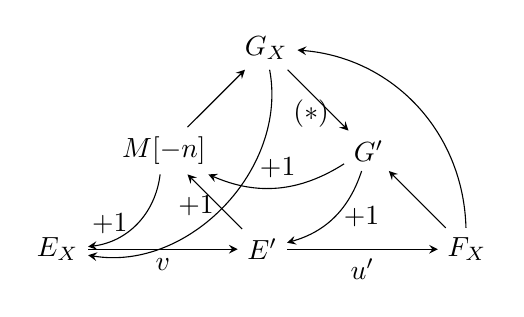
\begin{tikzpicture}[>=stealth,baseline=(GX.base),node distance=1.0cm]
  \node (EX) at (0,0) {$E_X$};
  \node (Ep) at (2.6,0) {$E'$};
  \node (FX) at (5.2,0) {$F_X$};
  \node (M)  at (1.35,1.25) {$M[-n]$};
  \node (GX) at (2.65,2.55) {$G_X$};
  \node (Gp) at (3.95,1.25) {$G'$};
  \node at (3.22,1.72) {$(*)$};
  \draw[->] (EX) -- node[below] {$v$} (Ep);
  \draw[->] (Ep) -- node[below] {$u'$} (FX);
  \draw[->] (Ep) -- (M);
  \draw[->] (M) -- (GX);
  \draw[->] (GX) -- (Gp);
  \draw[->] (FX) -- (Gp);
  \draw[->] (M) to[bend left=38] node[left] {$+1$} (EX);
  \draw[->] (Gp) to[bend left=28] node[above] {$+1$} (M);
  \draw[->] (Gp) to[bend left=28] node[right] {$+1$} (Ep);
  \draw[->] (GX) to[bend left=55] node[left] {$+1$} (EX);
  \draw[->] (FX) to[bend right=42] (GX);
\end{tikzpicture}
\]
La sucesión exacta de cohomología del triángulo distinguido \((*)\) muestra que \(\Ho^n(G_X)\longrightarrow \Ho^n(G')\) es un epimorfismo, por lo que \(\Ho^n(G')\) es efectivamente de \(\mathcal C_0\)-tipo finito.

La corrección anterior nos reduce, por tanto, al caso en que \(\Ho^{n+1}(u)\) es un monomorfismo, lo que supondremos en adelante. La sucesión exacta de cohomología de \(E\to F\to G\) da entonces una sucesión exacta
\begin{equation}\tag{.}
  \Ho^n(E)\xrightarrow{\Ho^n(u)}
  \Ho^n(F)\longrightarrow \Ho^n(G)\longrightarrow 0.
\end{equation}
Como \(\Ho^n(G)\) es de \(\mathcal C_0\)-tipo finito, el conjunto de los \(X\) sobre \(S\) tales que existe un epimorfismo \(M\longrightarrow \Ho^n(G_X)\), con \(M\in\Ob\mathcal C_{0,X}\), es, por definición, un refinamiento de \(S\). Utilizando la cuasilevantabilidad de \(\mathcal C_0\) en \(\mathcal C\), se puede imponer que este epimorfismo se factorice a través de \(Z^n(F_X)\) en
\[
  M\xrightarrow{s}Z^n(F_X)\longrightarrow \Ho^n(F_X)\longrightarrow \Ho^n(G_X).
\]
Está claro que \(u'\), definido como en (1.4.1) con \((r=0)\), es un morfismo de complejos y que \(\Ho^{n+1}(u')=\Ho^{n+1}(u_X)\). Por otra parte, es inmediato, a partir de la sucesión exacta (.), que
\[
  \Ho^n(u'):\Ho^n(E_X)\oplus M\longrightarrow \Ho^n(F_X)
\]
es un epimorfismo. Esto termina la demostración de (1.4.1).

\textbf{Lema 1.4.2.} \emph{Sean \(\mathcal C\) una categoría abeliana, \(u:E\to F\) un morfismo de complejos de \(\mathcal C\) (respectivamente, una flecha de \(\Dpx(\mathcal C)\)), y \(G\) el cono de \(u\). Para un \(n\in\mathbb Z\) dado, las condiciones siguientes son equivalentes}:
\begin{enumerate}[label=(\roman*)]
\item \emph{\(\Ho^i(G)=0\) para \(i\geq n\)}~;
\item \emph{\(\Ho^i(u)\) es un isomorfismo para \(i>n\) y un epimorfismo para \(i=n\)}.
\end{enumerate}
La demostración es inmediata a partir de la sucesión exacta de cohomología.

\textbf{Definición 1.4.3.} \emph{Diremos que \(u\) es un \(n\)-cuasi-isomorfismo (respectivamente, un \(n\)-isomorfismo) si \(u\) verifica las condiciones equivalentes de (1.4.2).}

Establecido esto, se deduce inmediatamente de (1.4.1) el

\textbf{Corolario 1.4.4.} \emph{Sean \(\sisi{S}{\mathcal S},S,\mathcal C,\mathcal C_0\) como en (1.4.1). Sea \(u:E\to F\) un \((n+1)\)-cuasi-isomorfismo de complejos de \(\mathcal C_S\) (para un \(n\in\mathbb Z\) dado), tal que \(\Ho^n(G)\) sea de \(\mathcal C_0\)-tipo finito. Entonces el conjunto de los \(X\) sobre \(S\) tales que existen \((M,r,s)\), como en (1.4.1), para los cuales \(u'\) es un \(n\)-cuasi-isomorfismo, es un refinamiento de \(S\).}

De manera figurada, bajo la condición de finitud sobre \(\Ho^n(G)\), se puede localmente «~ganar un grado~», es decir, modificar localmente \(u\) en grado \(n\), añadiendo a \(E^n\) un objeto de \(\mathcal C_0\), de manera que \(u\) se convierta en un \(n\)-cuasi-isomorfismo.

\textbf{Corolario 1.4.5.} Sean \(\mathcal C\) una categoría abeliana, \(n\in\mathbb Z\), y \(u:E\to F\) un \(n\)-cuasi-isomorfismo de complejos de \(\mathcal C\). Existe un diagrama conmutativo de \(\Cpx(\mathcal C)\)
\[
\begin{tikzcd}
E \arrow[r,"v"] \arrow[d,"u"'] & E' \arrow[dl,"u'"]\\
F &
\end{tikzcd}
\]
donde \(u'\) es un cuasi-isomorfismo y \(v\) un monomorfismo que induce la identidad en grado \(\geq n\) (es decir, tal que \(E'^i=E^i\) y \(v^i=\id(E^i)\) para \(i\geq n\)).

\emph{Demostración.} Aplicando (1.4.4) cuando \(\sisi{S}{\mathcal S}\) es el sitio puntual y \(\mathcal C_0=\mathcal C\), se obtiene un triángulo conmutativo de \(\Cpx(\mathcal C)\)
\[
\begin{tikzcd}
E \arrow[r,"v_{n-1}"] \arrow[d,"u"'] & E'_{\,n-1} \arrow[dl,"u'_{n-1}"]\\
F &
\end{tikzcd}
\]
donde \(u'_{n-1}\) es un \((n-1)\)-cuasi-isomorfismo y \(v_{n-1}\) un monomorfismo que induce la identidad en grado \(\geq n\). Iterando el procedimiento, se obtiene, para \(i\leq n-1\), una sucesión de triángulos conmutativos de \(\Cpx(\mathcal C)\)
\[
\begin{tikzcd}
E'_i \arrow[r,"v_{i-1}"] \arrow[d,"u'_i"'] & E'_{\,i-1} \arrow[dl,"u'_{i-1}"]\\
F &
\end{tikzcd}
\]
donde \(u'_i\) es un \(i\)-cuasi-isomorfismo y \(v_{i-1}\) un monomorfismo que induce la identidad en grado \(\geq i\). El corolario se deduce de ello por paso al límite. Con precisión, denotando por \(d'_i\) el diferencial de \(E'_i\), se define \(E'\) mediante
\[
  E'^i=E^i,\quad d'^i=d^i\quad\text{para }i\geq n,
\]
y
\[
  E'^i=(E'_i)^i,\quad d'^i=(d'_i)^i\quad\text{para }i<n,
\]
y luego \(v\) y \(u'\) mediante
\[
  v^j=(v_i)^j,\qquad u'^j=(u'_i)^j\qquad\text{para }i\leq j,
\]
y se comprueba inmediatamente que \(E'\), \(v\) y \(u'\), definidos de este modo, responden a lo pedido.

En otros términos, abreviadamente, se puede prolongar un \(n\)-cuasi-isomorfismo a un cuasi-isomorfismo «~sin cambiar nada de lo dado en grado \(\geq n\)~».
